\documentclass{article}
\usepackage[utf8]{inputenc}
\usepackage{amsmath,amssymb}
\usepackage{makecell}
\usepackage[a4paper, total={6in, 9in}]{geometry}
\usepackage{authblk}
\usepackage{graphicx}
\graphicspath{{.}}
\author{Zihan Zhao}
\affil{1001103708}
\title{Homework 2}
\date{}
\begin{document}
\maketitle
\section{}
\renewcommand{\thesubsection}{(\alph{subsection})}
\subsection{}
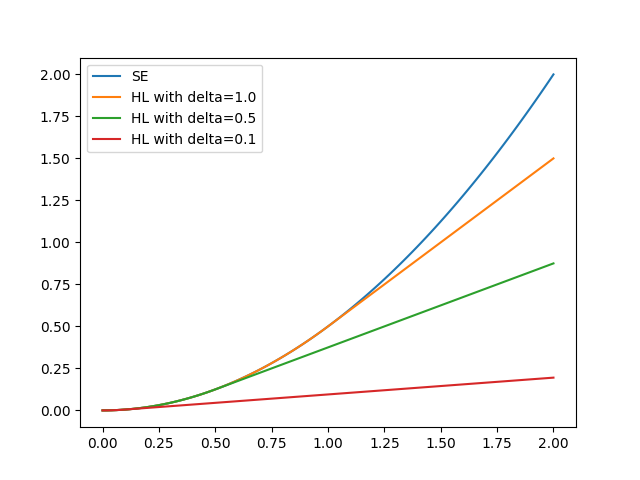
\includegraphics{q1a.png}
Compared with squared error loss, when the residue (y-t) increases, Huber loss is the same as squared error loss. But when it reaches over the threshold $\delta$, i.e. the loss is at outliers, Huber loss becomes linearly increasing by the slope of $\delta$. It becomes less sensitive to outliers than squared error loss. So the optimal weights can be determined more quickly by using Huber loss gradient descent. Therefore it is robust regression.
\subsection{}
Now determines $\frac{\mathrm{d} L_\delta}{\mathrm{d} w}$:
\begin{align*}
    \frac{\mathrm{d} L_\delta}{\mathrm{d} w}&=  \frac{\mathrm{d} H_\delta (a)}{\mathrm{d} a} \frac{\mathrm{d} a}{\mathrm{d} y}\frac{\mathrm{d} y}{\mathrm{d} w}\\
\intertext{When $|y-t| \leqq \delta$:}
    &= \frac{\mathrm{d} \frac{1}{2}a^2 }{\mathrm{d} a} \frac{\mathrm{d} a}{\mathrm{d} y} \frac{\mathrm{d} y}{\mathrm{d} w}\\
    &= a * 1 * x = ax = (y-t)x\\
    &= (w^\intercal x+b-t)x\\
\intertext{When $|y-t| > \delta$:}
    &= \frac{\mathrm{d} \delta(|a|-\frac{1}{2}\delta)}{\mathrm{d} a} \frac{\mathrm{d} a}{\mathrm{d} y} \frac{\mathrm{d} y}{\mathrm{d} w}\\
    &=
    \begin{cases}
    \delta x, &y-t>\delta\\
    -\delta x, &y-t<-\delta\\
    \end{cases}
\end{align*}
Now determines $\frac{\mathrm{d} L_\delta}{\mathrm{d} b}$:
\begin{align*}
    \frac{\mathrm{d} L_\delta}{\mathrm{d} b}&=  \frac{\mathrm{d} H_\delta (a)}{\mathrm{d} a} \frac{\mathrm{d} a}{\mathrm{d} y}\frac{\mathrm{d} y}{\mathrm{d} b}\\
\intertext{When $|y-t| \leqq \delta$:}
    &= \frac{\mathrm{d} \frac{1}{2}a^2 }{\mathrm{d} a} \frac{\mathrm{d} a}{\mathrm{d} y} \frac{\mathrm{d} y}{\mathrm{d} b}\\
    &= a * 1 * 1 = x\\
    &= w^\intercal x+b-t\\
\intertext{When $|y-t| > \delta$:}
    &= \frac{\mathrm{d} \delta(|a|-\frac{1}{2}\delta)}{\mathrm{d} a} \frac{\mathrm{d} a}{\mathrm{d} y} \frac{\mathrm{d} y}{\mathrm{d} w}\\
    &=
    \begin{cases}
    \delta , &y-t>\delta\\
    -\delta , &y-t<-\delta\\
    \end{cases}
\end{align*}
\subsection{}
Look at q1.py.
\section{}
\subsection{}
First factor the Loss formula:
\begin{align*}
    L &= \frac{1}{2}\sum_{i = 1}^{N} a^{(i)} (y^{(i)} - w^\intercal x^{(i)} )^2 + \frac{\lambda}{2}||w||^2 \\
    &= \frac{1}{2}A||Y-Xw||^2 + \frac{\lambda}{2}w^\intercal w \; \text{(where Y is Nx1, X is Nxd, A is NxN, and w is dx1)}\\
    &= \frac{1}{2}(Y-Xw)^\intercal (A(Y-Xw)) + \frac{\lambda}{2}w^\intercal w\\
    &= \frac{1}{2}(Y^\intercal AY-Y^\intercal AXw -(Xw)^\intercal AY + w^\intercal X^\intercal AXw) + \frac{\lambda}{2}w^\intercal w\\
    &= \frac{1}{2}(Y^\intercal AY-Y^\intercal AXw - (AY)^\intercal Xw + w^\intercal (X^\intercal AX)w) + \frac{\lambda}{2}w^\intercal w\\
    &= \frac{1}{2}(Y^\intercal AY-Y^\intercal AXw - Y^\intercal A^\intercal Xw + w^\intercal (X^\intercal AX)w) + \frac{\lambda}{2}w^\intercal w\\
\intertext{Since $A = A^\intercal$,}
    &= \frac{1}{2}(Y^\intercal AY-Y^\intercal AXw - Y^\intercal AXw + w^\intercal (X^\intercal AX)w) + \frac{\lambda}{2}w^\intercal w\\
    &= \frac{1}{2}Y^\intercal AY-Y^\intercal AXw + \frac{1}{2}w^\intercal (X^\intercal AX)w + \frac{\lambda}{2}w^\intercal w\\
\end{align*}
Now take derivative of L by w:
\begin{align*}
\intertext{Since $A = A^\intercal$, so $X^\intercal AX$ is symmatric as well, then}
    \frac{\mathrm{d} L}{\mathrm{d} w} &= 0-Y^\intercal AX + \frac{1}{2}2(X^\intercal AX)w + \frac{1}{2}2\lambda w\\
    &= -Y^\intercal AX  + (X^\intercal AX)w + \lambda w\\
\intertext{Let $\frac{\mathrm{d} L}{\mathrm{d} w} = 0$, we got}
-Y^\intercal AX  + (X^\intercal AX)w + \lambda w &= 0\\
(X^\intercal AX + \lambda I)w &= Y^\intercal AX\\
w &= (X^\intercal AX + \lambda I)^{-1}Y^\intercal AX\\
\intertext{Since $Y^\intercal AX = (AX)^\intercal Y = X^\intercal A^\intercal Y = X^\intercal A Y$,}
w &= (X^\intercal AX + \lambda I)^{-1}X^\intercal AY\\
\end{align*}
Done.
\subsection{}
Look at q2.py.
\subsection{}
Look at q2.py.
\end{document}
